\chapter{Project Premise and Model Design} 

\section{Premise}

%TODO: need to discuss ferry characteristics - task oriented


Message ferrying, also known as store-carry-forward, is the approach of physically carrying data from nodes that are out of range and deliver them to their destination. 
Some of the advantages of message ferries are that they virtually do not require physical infrastructure and that they also have a low cost. 

	
\subsection{Application Characteristics and Requirements}

Any application running over a message ferrying network must have the following characteristics:

\begin{description}
\item[Delay Tolerance: ]
Since data is transported by a physical device, significant delays of minutes to hours must be expected.
\item[Loss Tolerance: ]
Given that ferries have limited memory, loss of data must be expected.
\item[Small and Independent Messages: ]
Following from the limited memory capacity of ferries and the high probability of packet loss, a reliable method for segmentation and reassembly of messages should not be expected. 
Applications should limit the size of messages such that the can be transmitted in their entirety using one network packet.
%Use PDU instead of packet?
%
(See section \ref{sec:fountain_codes} for future work)
\end{description}

Given these criteria, a message ferrying network is unsuitable for many typical networking applications including web browsing, real-time voice or text communication and file transfer.
As such, a very specialized 'state monitoring' network designed for non-critical monitoring of remote sensors is considered.

\subsection{State Monitoring Network}

The general premise for this project consists of a network containing numerous, uniquely identifiable source nodes. 
Each source node has a limited number of properties, in the form of key/value pairs, specifying a property name (the key) and its current value.
Properties may change overtime and each change defines a new state for the source node.
A temperature sensor for example, might support a 'temperature' property, the value of which is the current temperature updated every hour.
Properties do not have to contain a single value and each may be as large as the payload limit of network packets. %Somewhat of a vague statement

%TODO: introduction to node types
%	Perhaps put in the Network Elements section below
%
%This needs to be broken into an new section or placed in a subsection



%TODO: new section

The network and message ferrying algorithm is designed to synchronize a central repository with the current state of every source node.
Only the most recent state (or most recent value) for each property is important, not the history of how that property has changed.
This limits the number of packets which can exist in the network as only the most recent update must be reported.
%The significance of this characteristic is described below. 
The message ferries collect data from source nodes when they are in range and transport it to the central repository.
The central repository is assumed to be a server connected to the Internet.
Ferries pass updates they have collected from source nodes to special gateway nodes.
These gateway nodes are then responsible for using a reliable delivery mechanism over a standard IP network to update the central repository.

\emph{Insert image showing this process.}

%--------------------------------------------------------------------------------------------------------
% 		Design
%--------------------------------------------------------------------------------------------------------
\section{Model Design}
\subsection{Network Elements}


%This section describes the elements present in the network.

\subsubsection{Nodes}

The network is comprised of three types of nodes:

\begin{description}

\item[Source Node: ] 
Static nodes in the network which have a set of properties (key/value pairs).
After a property of a source changes, known as a state change, it attempt to notify the central repository by transferring update packets to message ferries.
A source node could be, for example, a remote temperature sensor.
\item[Message Ferry: ] 
A mobile node which collects updates from source nodes when they are in range.
Message ferries store update packets from source nodes within a buffer. 
When in range, these update packets are forwarded to gateway nodes.
A source node could be, for example, a specially equipt cell phone or a small computer attached to a vehicle. 
\item[Gateway: ]
Gateway nodes download update packets form message ferries and forward them to the central repository over the Internet.
Transfer of updates between the gateway and central repository is assumed to be reliable. 

\end{description}


Sources have properties (prop1, prop2, etc) which generate messages. These messages get carried to any gateway node by message ferries.

\begin{figure}[h]
    \centering
    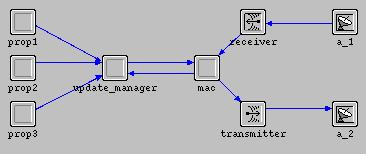
\includegraphics[width=.5\textwidth]{images/source}
    \caption{Source Node Model}
    \label{fig:source}
\end{figure}

Source node shown in figure \ref{fig:source} is a static node in the network which have a set of properties that generate update messages. The three properties shown in the figure generate updates and the mac process controls wireless access. 	

%\item[Central Repository: ] 
%The central repository is a server and the final destination for updates sent from source nodes.
%It maintains a list of the current state of all source nodes.
%There is only one central repository node.


\begin{figure}[h]
    \centering
    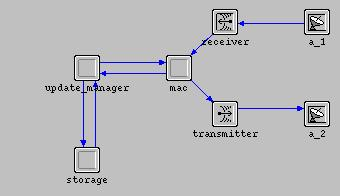
\includegraphics[width=.5\textwidth]{images/ferry}
    \caption{Ferry Node}
    \label{fig:Ferry}
\end{figure}

Ferry Node shown in figure \ref{fig:Ferry} is a mobile node which collects updates from source nodes when they are in range. These updates are then stored in memory. The storage process compares the updates and keeps the most recent according to the key update. It also checks which update to keep and gets rid of the older ones.

\begin{figure}[h]
    \centering
    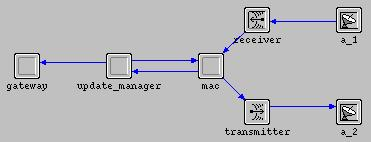
\includegraphics[width=.5\textwidth]{images/gateway}
    \caption{Gateway Node}
    \label{fig:Gateway}
\end{figure}

Gateway Node shown in figure \ref{fig:Gateway} receives the update messages from ferries and forwards them to their final destination via the Internet. Gateway process records the updates.



\subsubsection{Properties}

Source node has three main pieces of data:
\begin{itemize}
\item Source ID
\item Key
\item Key update number
\end{itemize}

Note that the key update number is extremely important because it lets the ferry know of the most recent update.


\subsubsection{Packets}

At the network layer, two types of packets are used as follows:

\begin{description}
\item[Update Packet: ]
Update packets are generated by source nodes when a message ferry is in range and their state has changed. 
Source nodes will continue to generate update packets until the state change is acknowledged by the central repository (using an acknowledgment packet).
\item[Beacon Packet: ] 
Beacon packets are first generated by ferry nodes to discover if there are source nodes in range. 
When there are source nodes in range, they give their updates to the ferries. Similar procedure happens between the ferry and source nodes. 
%TODO:  Why range is 60m
\end{description}

%--------------------------------------------------------------------------------------------------------
% 		Algorithm
%--------------------------------------------------------------------------------------------------------
\subsection{Algorithm and Behavior - Simplified}

\subsubsection{Ferry Algorithm}

Ferry nodes do the steps shown below in order:

\begin{enumerate}
\item Move around sending beacons to notify other nodes that there is a ferry in range.
\item When a source node is in range, the ferry node receives the updates from it.
\item Ferry nodes only keep the most recent update according to the key update number and age.
	\begin{enumerate}
	\item It compares the updates and keeps the most recent according to the key update.
	\item If a ferry gets full, it considers the age and gets rid of the oldest update
	\end{enumerate}
\item It then moves till a gateway beacon is received.
\item Ferry node then sends the updates to the gateway.
\end{enumerate}

\subsubsection{Source Algorithm}

Source nodes do the steps shown below in order:

\begin{enumerate}
\item They wait till a beacon is receive from the ferry node.
\item Based on the current state, key update,  they send three properties to the ferry node.

\end{enumerate}


\subsubsection{Gateway Algorithm}

Gateway nodes do the steps shown below in order:

\begin{enumerate}
\item Gateway nodes notify ferries that there's a beacon in range.
\item Ferries then send their most recent update to the gateway nodes.
\item Gateway nodes receives these updates.
\item Records that an update has been received.
\end{enumerate}


\subsection{Assumptions}

There were assumptions made to prevent the complexity they would have caused.

\begin{itemize}
\item Communication range of 60m:
	This means that only nodes within that range can communicate. 

\item No propagation and transmission delay:
	These might happen when a ferry node goes by quicker and can't catch everything in time. 
	
\item No unintentional loss:
	We assume that there is no loss caused by interference. We're assuming that any loss that happens is 			intentional.
	
	
\end{itemize}

Note that now there are technologies that provide solutions to the problems noted above. 

%--------------------------------------------------------------------------------------------------------
% 		Other stuff to include
%--------------------------------------------------------------------------------------------------------




% TODO	- Major improvement -> better mac

%This section needs to be changed a lot
%Lets break it down into 'validation' and put that in the previous section
%
%I am adding another section which talks about the 'main' simulation

\section{Validation} %TODO: no longer a chapter

%small intro
In this section, we will discuss the simulation to validate our design and implementation. 
A scenario is created to validate that the updates from source nodes are delivered successfully when in range to the ferry node and the update packets are handled properly by the ferry node as designed.   
Further detail will be explained in the following subsequent section \ref{sec:scenario1}. %might remove this line


%When simulating each scenario, the following metrics will be measured:
%\begin{enumerate}
%	\item Time to update state in central repository (delay)
%	\item Variation in time to update state (delay jitter)
%	\item Number of state updates lost. Roughly corresponds to packet loss.
%	\item Memory utilization and packet dropping threshold within ferries.
%\end{enumerate}

%_________________________________________________________________
%________________________SCENARIO 1_______________________________
\subsection{Scenario Topology  and Details}
\label{sec:scenario1}


In Figure \ref{fig:scenario1}, it shows the topology to test if the gateway receives the update packets sent by the source nodes and if the ferry is picking up these update packets from source nodes when it moves past them.
There is one gateway node, one ferry node, and seven source nodes. 
The size of this topology is 0.75km x 0.75km with source nodes placed evenly apart by 0.375km. 
The gateway node is on the top left corner, and the ferry is in motion indicated next to a red arrow.
The speed of the ferry is a constant 60kph, as it moves clockwise two times along the rectangular path that is highlighted in white.  The simulated time is six minutes.

%picture of the rectangular path
\begin{figure}[ht]
    \centering
    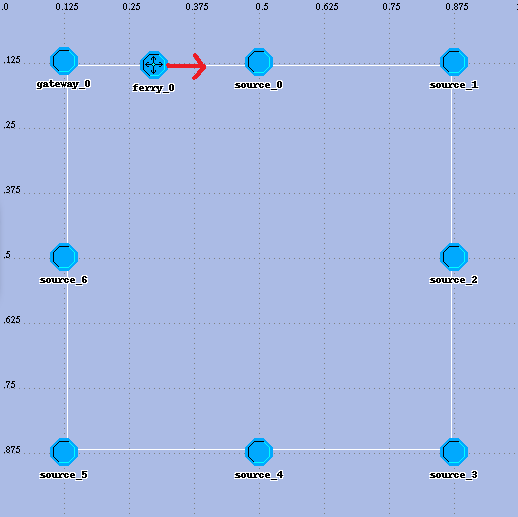
\includegraphics[width=.5\textwidth]{images/scenario1-top1r}
    \caption{Validation scenario topology}
    \label{fig:scenario1}
\end{figure}

\subsection{Validation Simulation Results}
\label{sec:results-validate}


After setting up OPNET to capture the desired statistics, the design and implementation are simulated.  The results are collected and shown in Figure \ref{fig:result1-a}.  From it, we can see that the ferry is picking up three update packets each time it passes by a source node.  This validates that ......

%result1-a   ferry receives update packets
\begin{figure}[ht]
    \centering
    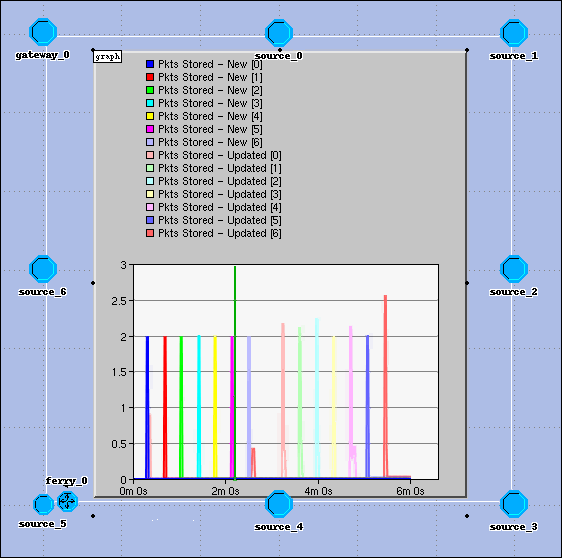
\includegraphics[width=.5\textwidth]{images/scenario1-result-received}
    \caption{Update packets received by the fery node}
    \label{fig:result1-a}
\end{figure}

The second part of the results is to see the if the gateway receives the update packets collected by the ferry node.  From Figure \ref{fig:result1-b}, there are two spikes in the graph which corresponds to the task of dumping the packets to the gateway node.  
The ferry node goes around two times for this simulation and that is why we see we two spikes.  
Each source node sends three update packets to the ferry node as it passes.  
Since there are seven source nodes, this accounts for the 20 packets received by the gateway node, which can be seen in Figure \ref{fig:result1-b}.


%result1-b   ferry delivers update packets to gateway
\begin{figure}[ht]
    \centering
    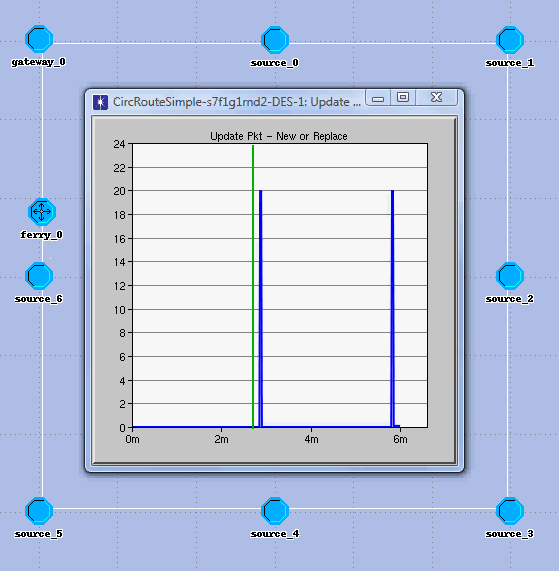
\includegraphics[width=.5\textwidth]{images/scenario1-result-gateway}
    \caption{Gateway receives the packet as the ferry node passes by its range of transmission}
    \label{fig:result1-b}
\end{figure}

